

\tikzset{every picture/.style={line width=1.05pt}} %set default line width to 0.75pt        

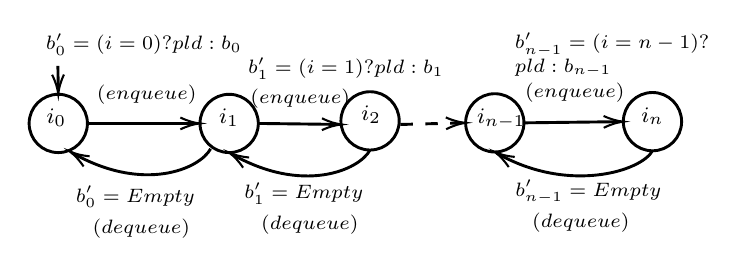
\begin{tikzpicture}[x=0.65pt,y=0.65pt,yscale=-1,xscale=1]
%uncomment if require: \path (0,300); %set diagram left start at 0, and has height of 300


%Shape: Circle [id:dp31914676096119765] 
\draw   (74.6,98.1) .. controls (74.6,89.15) and (81.85,81.9) .. (90.8,81.9) .. controls (99.75,81.9) and (107,89.15) .. (107,98.1) .. controls (107,107.05) and (99.75,114.3) .. (90.8,114.3) .. controls (81.85,114.3) and (74.6,107.05) .. (74.6,98.1) -- cycle ;
%Straight Lines [id:da37317958939159324] 
\draw    (90.6,66.13) -- (90.78,79.9) ;
\draw [shift={(90.8,81.9)}, rotate = 269.29] [color={rgb, 255:red, 0; green, 0; blue, 0 }  ][line width=0.75]    (10.93,-3.29) .. controls (6.95,-1.4) and (3.31,-0.3) .. (0,0) .. controls (3.31,0.3) and (6.95,1.4) .. (10.93,3.29)   ;
%Shape: Circle [id:dp22901745321019074] 
\draw   (169.6,98.1) .. controls (169.6,89.15) and (176.85,81.9) .. (185.8,81.9) .. controls (194.75,81.9) and (202,89.15) .. (202,98.1) .. controls (202,107.05) and (194.75,114.3) .. (185.8,114.3) .. controls (176.85,114.3) and (169.6,107.05) .. (169.6,98.1) -- cycle ;
%Shape: Circle [id:dp6850049335985016] 
\draw   (317.27,97.77) .. controls (317.27,88.82) and (324.52,81.57) .. (333.47,81.57) .. controls (342.41,81.57) and (349.67,88.82) .. (349.67,97.77) .. controls (349.67,106.71) and (342.41,113.97) .. (333.47,113.97) .. controls (324.52,113.97) and (317.27,106.71) .. (317.27,97.77) -- cycle ;
%Straight Lines [id:da10806683009608209] 
\draw    (107,98.1) -- (167.6,98.1) ;
\draw [shift={(169.6,98.1)}, rotate = 180] [color={rgb, 255:red, 0; green, 0; blue, 0 }  ][line width=0.75]    (10.93,-3.29) .. controls (6.95,-1.4) and (3.31,-0.3) .. (0,0) .. controls (3.31,0.3) and (6.95,1.4) .. (10.93,3.29)   ;
%Straight Lines [id:da8217014567182165] 
\draw  [dash pattern={on 4.5pt off 4.5pt}]  (281,98.67) -- (315.27,97.82) ;
\draw [shift={(317.27,97.77)}, rotate = 178.58] [color={rgb, 255:red, 0; green, 0; blue, 0 }  ][line width=0.75]    (10.93,-3.29) .. controls (6.95,-1.4) and (3.31,-0.3) .. (0,0) .. controls (3.31,0.3) and (6.95,1.4) .. (10.93,3.29)   ;
%Shape: Circle [id:dp08560151992011589] 
\draw   (247.93,96.67) .. controls (247.93,87.72) and (255.19,80.47) .. (264.13,80.47) .. controls (273.08,80.47) and (280.33,87.72) .. (280.33,96.67) .. controls (280.33,105.61) and (273.08,112.87) .. (264.13,112.87) .. controls (255.19,112.87) and (247.93,105.61) .. (247.93,96.67) -- cycle ;
%Straight Lines [id:da7410245959347421] 
\draw    (202,98.1) -- (246.33,98.64) ;
\draw [shift={(248.33,98.67)}, rotate = 180.7] [color={rgb, 255:red, 0; green, 0; blue, 0 }  ][line width=0.75]    (10.93,-3.29) .. controls (6.95,-1.4) and (3.31,-0.3) .. (0,0) .. controls (3.31,0.3) and (6.95,1.4) .. (10.93,3.29)   ;
%Shape: Circle [id:dp4984227004498517] 
\draw   (404.93,97.1) .. controls (404.93,88.15) and (412.19,80.9) .. (421.13,80.9) .. controls (430.08,80.9) and (437.33,88.15) .. (437.33,97.1) .. controls (437.33,106.05) and (430.08,113.3) .. (421.13,113.3) .. controls (412.19,113.3) and (404.93,106.05) .. (404.93,97.1) -- cycle ;
%Straight Lines [id:da9002692791455889] 
\draw    (349.67,97.77) -- (402.93,97.12) ;
\draw [shift={(404.93,97.1)}, rotate = 179.31] [color={rgb, 255:red, 0; green, 0; blue, 0 }  ][line width=0.75]    (10.93,-3.29) .. controls (6.95,-1.4) and (3.31,-0.3) .. (0,0) .. controls (3.31,0.3) and (6.95,1.4) .. (10.93,3.29)   ;
%Curve Lines [id:da054067545547898055] 
\draw    (421.13,113.3) .. controls (415.06,124.55) and (374.49,137.41) .. (334.67,114.67) ;
\draw [shift={(333.47,113.97)}, rotate = 30.52] [color={rgb, 255:red, 0; green, 0; blue, 0 }  ][line width=0.75]    (10.93,-3.29) .. controls (6.95,-1.4) and (3.31,-0.3) .. (0,0) .. controls (3.31,0.3) and (6.95,1.4) .. (10.93,3.29)   ;
%Curve Lines [id:da19389154071839954] 
\draw    (264.13,112.87) .. controls (258.06,124.12) and (226.64,137.72) .. (187,115) ;
\draw [shift={(185.8,114.3)}, rotate = 30.52] [color={rgb, 255:red, 0; green, 0; blue, 0 }  ][line width=0.75]    (10.93,-3.29) .. controls (6.95,-1.4) and (3.31,-0.3) .. (0,0) .. controls (3.31,0.3) and (6.95,1.4) .. (10.93,3.29)   ;
%Curve Lines [id:da5969865187078301] 
\draw    (175.47,112.2) .. controls (169.39,123.45) and (137.97,137.06) .. (98.34,114.33) ;
\draw [shift={(97.13,113.63)}, rotate = 30.52] [color={rgb, 255:red, 0; green, 0; blue, 0 }  ][line width=0.75]    (10.93,-3.29) .. controls (6.95,-1.4) and (3.31,-0.3) .. (0,0) .. controls (3.31,0.3) and (6.95,1.4) .. (10.93,3.29)   ;


% Text Node
\draw (108,149) node [anchor=north west][inner sep=0.75pt]  [font=\scriptsize]  {$( dequeue)$};
% Text Node
\draw (98.67,131) node [anchor=north west][inner sep=0.75pt]  [font=\scriptsize]  {$b_{0} '=Empty$};
% Text Node
\draw (201.67,147) node [anchor=north west][inner sep=0.75pt]  [font=\scriptsize]  {$( dequeue)$};
% Text Node
\draw (192.33,129) node [anchor=north west][inner sep=0.75pt]  [font=\scriptsize]  {$b_{1} '=Empty$};
% Text Node
\draw (352.33,145.67) node [anchor=north west][inner sep=0.75pt]  [font=\scriptsize]  {$( dequeue)$};
% Text Node
\draw (348.33,73.67) node [anchor=north west][inner sep=0.75pt]  [font=\scriptsize]  {$( enqueue)$};
% Text Node
\draw (335,45.67) node [anchor=north west][inner sep=0.75pt]  [font=\scriptsize]  {$ \begin{array}{l}
b_{n-1} '=( i=n-1) ?\\
pld:b_{n-1}
\end{array}$};
% Text Node
\draw (413,87.33) node [anchor=north west][inner sep=0.75pt]  [font=\footnotesize]  {$i_{n}$};
% Text Node
\draw (257.33,86.33) node [anchor=north west][inner sep=0.75pt]  [font=\footnotesize]  {$i_{2}$};
% Text Node
\draw (343,127.67) node [anchor=north west][inner sep=0.75pt]  [font=\scriptsize]  {$b_{n-1} '=Empty$};
% Text Node
\draw (195.67,77) node [anchor=north west][inner sep=0.75pt]  [font=\scriptsize]  {$( enqueue)$};
% Text Node
\draw (194.33,59.67) node [anchor=north west][inner sep=0.75pt]  [font=\scriptsize]  {$b_{1} '=( i=1) ?pld:b_{1}$};
% Text Node
\draw (82,46.33) node [anchor=north west][inner sep=0.75pt]  [font=\scriptsize]  {$b_{0} '=( i=0) ?pld:b_{0}$};
% Text Node
\draw (110.33,74.67) node [anchor=north west][inner sep=0.75pt]  [font=\scriptsize]  {$( enqueue)$};
% Text Node
\draw (321.67,88) node [anchor=north west][inner sep=0.75pt]  [font=\footnotesize]  {$i_{n-1}$};
% Text Node
\draw (178.33,88) node [anchor=north west][inner sep=0.75pt]  [font=\footnotesize]  {$i_{1}$};
% Text Node
\draw (82.33,88) node [anchor=north west][inner sep=0.75pt]  [font=\footnotesize]  {$i_{0}$};


\end{tikzpicture}